% REMEMBER: You must not plagiarise anything in your report. Be extremely careful.

\documentclass{l4proj}


    
%
% put any additional packages here
%

\begin{document}

%==============================================================================
%% METADATA
\title{Thrive: Promoting physical activity for mental well-being}
\author{Andy Lopez Suarez}
\date{April, 2022}

\maketitle
%==============================================================================
%% ABSTRACT
\begin{abstract}
Globally, over the last decade, we have seen a concerning increase in sedentary behavior in our modern world. This has only further increased with the occurrence of the COVID-19 pandemic, which has acted as a catalyst in increasing sedentary behavior. The pandemic has profoundly impacted the mental health of the public. While the government has employed different methods to ease the impact on the health services as they focus on coping with COVID-19, different strategies need to be explored to address the new mental health crisis. 

Fitness trackers have become a fashionable way to promote physical activity in people. While these have shown to be effective, many of these commercial fitness trackers do not make use of novel techniques that have been proven to increase physical activity. In this project, these techniques have been applied to create a gamified mobile application titled Thrive. It allows individuals to work within a team to achieve collaborative and individual goals. Whether this mobile fitness tracker positively impacts the mental well-being of an individual was analyzed in this project and concluded that this was indeed the case. This further recognizes that there exists a positive relationship between regular physical activity and mental well-being. The real-life implications of this outcome mean that individuals can benefit long-term and short-term from doing routine physical activity by using similar mobile fitness applications.

\end{abstract}

%==============================================================================

% EDUCATION REUSE CONSENT FORM
% If you consent to your project being shown to future students for educational purposes
% then insert your name and the date below to  sign the education use form that appears in the front of the document. 
% You must explicitly give consent if you wish to do so.
% If you sign, your project may be included in the Hall of Fame if it scores particularly highly.
%
% Please note that you are under no obligation to sign 
% this declaration, but doing so would help future students.
%
%\def\consentname {} % your full name
%\def\consentdate {} % the date you agree
%
\educationalconsent


%==============================================================================
\tableofcontents

%==============================================================================
%% Notes on formatting
%==============================================================================
% The first page, abstract and table of contents are numbered using Roman numerals and are not
% included in the page count. 
%
% From now on pages are numbered
% using Arabic numerals. Therefore, immediately after the first call to \chapter we need the call
% \pagenumbering{arabic} and this should be called once only in the document. 
%
% Do not alter the bibliography style.
%
% The first Chapter should then be on page 1. You are allowed 40 pages for a 40 credit project and 30 pages for a 
% 20 credit report. This includes everything numbered in Arabic numerals (excluding front matter) up
% to but excluding the appendices and bibliography.
%
% You must not alter text size (it is currently 10pt) or alter margins or spacing.
%
%
%==================================================================================================================================
%
% IMPORTANT
% The chapter headings here are **suggestions**. You don't have to follow this model if
% it doesn't fit your project. Every project should have an introduction and conclusion,
% however. 
%
%==================================================================================================================================

\chapter{Introduction}

% reset page numbering. Don't remove this!
\pagenumbering{arabic} 



\section{Motivation}
Fitness trackers have become popular with the public over the last decade, from the release of the wearable Fitbit in 2014 to the Tokyo 2020 Olympic games, where archers broadcasted their heart rates live on TV. At the same time, while these trackers have shown to be effective in supporting physical activity by the work of Laranjo et al. (2021), most of these limit themselves to only focusing on tracking an individual’s health data. They ignore the added benefits that arise from including collaborative and gamified features in fitness trackers. \vskip 0.5em

Over the last two decades, we have seen an increase in sedentary behavior globally [\citenum{2}] due to our modernized world, with 85\% of people worldwide categorized as living a sedentary lifestyle [\citenum{3}]. People can now widely access motorized transport, and with technology innovations, it means that adults are increasingly finding themselves spending prolonged time sitting down in front of screens. The World Health Organization (WHO) warns that this shift in physical inactivity comes with concerning health risks such as doubling the danger of cardiovascular disease and increasing the risk of mental health problems. 
\vskip 0.5em
Over the last two years, with the spread of the COVID-19 virus, the world has seen an unprecedented impact on the public's physical and mental health. The pandemic has disrupted our already sedentary lifestyle and has further decreased physical activity with the introduction of working from home and remote learning. Sallis et al. (2021)[\citenum{4}] has recognized the need for administrations to promote physical activity to mitigate the severity of the COVID-19 virus in individuals. Furthermore, increased physical activity has shown to be an effective way to improve mental wellbeing- an important finding that can alleviate the mental health crisis that has emerged from the COVID-19 pandemic [\citenum{5}].

\section{Aims}
In light of the above motivations, the objective of this project was to create a mobile application fitness tracker that promotes routine physical activity by using collaborative and gamified techniques. By implementing these techniques, the project hopes to improve an individual’s physical activity levels and positively impact their mental wellbeing.
Here are the main objectives identified for the project: 

\begin{itemize}
\item Implement a system that allows an individual to track their physical activity 
\item Review effective behavioural change interventions methods to support an individual, so they adopt healthy fitness habits 
\item Implement a system that allows collaboration and sets a collective goal that a team can achieve by working together 
\item Evaluate the impact on mental wellbeing after using the mobile application by using the Warwick-Edinburgh Mental Wellbeing Scale
\end{itemize}

\section{Outline}
The following is an overview of the dissertation structure. 
\begin{itemize}
\item Chapter 2 Background: This chapter discusses the impact of Covid-19 and reviews existing fitness trackers.  
\item Chapter 3 Requirements Gathering: This chapter discusses the requirements of the system. 
\item Chapter 4 Design: This chapter discusses the design decisions made for the various iterations.
\item Chapter 5 Implementation: This chapter discusses in detail how the system was implemented.
\item Chapter 6 Evaluation: This chapter discusses the results and considers future work.
\item Chapter 7 Conclusion: This chapter summarises the main findings of the project. 
\end{itemize}

\chapter{Background}
This chapter discusses a range of existing fitness trackers that used different novel approaches to get a consumer to adopt healthy habits. The effectiveness of their techniques, their shortcomings, and how effective they were in promoting physical activity was examined. This would help select characteristics to adopt in the mobile application to promote physical activity effectively. Furthermore, what impact the COVID-19 pandemic has had on the physical and mental wellbeing of the public was reviewed. 

\section{COVID-19 Pandemic  }
Since the start of the COVID-19 pandemic over two years ago, it has had unprecedented consequences on the public's health worldwide and continues to disrupt many people's lives. People of all age groups have felt these consequences. Ranging from children whose childhood development has been negatively impacted [\citenum{6}] to both adolescents and adults alike struggling with increases in depression and anxiety [\citenum{7,8}], and to the elderly who have experienced a decrease in mobility and cognitive abilities due to having their daily routine disrupted [\citenum{9}].


\textbf{Mental health impact of COVID-19} \vskip 0.5em
Since the initial wave of the pandemic, the NHS has been left struggling to cope with the emerging mental health crisis alongside managing the virus. The UK population has experienced a significant rise in mental health problems (mainly seen in women, young adults, and vulnerable adults), with a 51\% increase in depression among adults reported in 2021 [\citenum{10}]. The UK government has launched campaigns throughout the country to mitigate the effects on public mental health and alleviate the pressure on the healthcare system. They focus on supporting mental health in the population, such as the “Clear Your Head “ Scottish campaign. Using multiple forms of media outlets, the campaign encourages the public to be mindful of their mental health by adopting healthy habits such as getting active, seeking support from friends and family, and improving sleep patterns [\citenum{11}]. 


\textbf{Physical health impact of COVID-19 }\vskip 0.5em
To reduce the spread of the virus in public, the UK government issued guidance to allow non-essential workers and students, where possible, to work or learn from home full-time [\citenum{12,3}]. This would help reduce the need to use public transport by cutting out the need to commute to workplaces or educational institutes. While this had a positive effect on flattening the curve, it had a negative impact on physical activity. Xiao et al. (2020) [\citenum{14}] reveal how adhering to these government policies inadvertently increased sedentary behavior and unhealthy eating habits. Moreover, there is a key relationship between regular physical activity and the severity of COVID-19, in which those that achieved more than 10 minutes of weekly activity decreased their mortality rate and their chances of being hospitalized with COVID-19 [\citenum{15}].




\textbf{Relation between physical and mental health }\vskip 0.5em
A UK study conducted by Jacob et al. (2020) [\citenum{16}] observed that adults who maintained high levels of physical activity during the pandemic experienced better overall mental health than their counterparts who experienced moderate to severe levels of anxiety and depression. To combat this, the UK government has issued nationwide campaigns to promote physical activity and mental wellbeing to help the healthcare system cope. This is an effective way to tackle the rise in mental health problems in the general public because there exists a positive relationship between physical activity and mental health. Regular physical activity has been proven to significantly reduce depression and anxiety by releasing endorphins [\citenum{17}]. Furthermore, the WHO recognizes that regular physical activity offers a variety of health benefits like reducing the risk of chronic disease, Alzheimer’s disease, and mortality rate.
 

\section{Fitness trackers}
\textbf{Effectiveness of mobile applications }\vskip 0.5em
Schoeppe et al. (2016) [\citenum{18}] reviewed a variety of mobile health applications and found they are effective in improving behavior, such as improving diet, physical activity, and sedentary behavior. Most notable, they saw the greatest improvement in physical activity among adults who did very low quantities of weekly physical activity. 


\textbf{Active 10 }\vskip 0.5em
The Active 10 mobile application is a fitness tracker designed by the NHS that aims to promote regular physical activity for at-risk user groups that do less than 30 minutes of weekly activity. Ciravegna et al. (2019) [\citenum{19}] describe how this population is at a higher risk of chronic disease and mental health problems, like depression and anxiety, which would negatively impact the healthcare system.  
To encourage the target user group to get active, the application sets 10-minute walking intervals to be completed by the user. This interval was selected as it is the minimum weekly amount of physical activity needed to be accomplished in order to start receiving health benefits [\citenum{20}]. The activity tracked was brisk walking and was chosen due to it being the most common form of aerobic exercise. Walking is recommended by WHO as one of the aerobic exercises that counts towards a person’s target weekly physical activity of 150 minutes, or daily 
physical activity of around 30 minutes. 
To support behavioral changes in an individual, the fitness application uses three proven features grounded in psychology. It gives users feedback and rewards, and lets user defines their own goals. These are effective behavior change interventions outlined by Wood et al. (2015) [\citenum{21}], who researched health intervention techniques for smoking cessation. 
The evaluation conducted revealed that the tracker was effective in increasing physical activity, with 54\% of their target group achieving a daily 10-minute walk after two months- a significant increase from less than 30 minutes of weekly activity. A limitation of the tracker being designed for at-risk user groups is that it does not accommodate active users that exercise beyond the daily 30-minute interval. 


\section{Gamified Fitness trackers }

\textbf{Zombies, Run! 5K Training}\vskip 0.5em
Zombies, Run! is an exergame that uses audio to deliver a storyline that utilizes psychological motivation to get users to run away from zombies. A health benefit of this application is that it motivates a user to exercise at different activity levels by switching between moderate and intensive physical activity according to the audio narrative. This is recognized by the WHO to give higher health benefits compared to only doing one moderate physical activity such as walking [\citenum{22}]. This application is targeted at users that want to get more active by gradually increasing the distance ran over a period of 8 weeks, where they will finally be able to run 5K. The application follows the principle of setting attainable goals to foster new physical activity in a user. A study conducted by Moran \& Coons (2015) [\citenum{23}] showed that the psychological motivation of being chased was effective in getting users to get active. Additionally, the design of the application consistently applies the theme of surviving the zombie apocalypse throughout the screens, through the color scheme and visual elements, to fully immerse the user in the exergame. A downside of the application is that the application only appeals to a limited user group.


\textbf{BunnyBolt}\vskip 0.5em
BunnyBolt [\citenum{24}] is an exergame mobile application that was designed for an adolescent user group. It incorporates a storyline that is less intensive compared to Zombies, Run! to be user-friendly to all age groups. It uses the element of gamification to appeal to and support the younger population to adopt healthy lifestyle habits. The application makes use of the 10-minute interval and a chasing element to get a user to be active. The application is visually engaging through its use of colors and fun elements to further appeal to their demographic. 

\section{Collaborative Fitness trackers }

\textbf {Pass the Ball}\vskip 0.5em
Pass the Ball [\citenum{25}] is a collaborative, competitive mobile application developed to track physical activity. To encourage collaboration within a team, it uses a novel approach of turn-taking within a team- it only tracks the physical activity of the player that has the ball. Creating a community to encourage physical activity motivates and benefits a person to a greater extent than taking an individual approach which is less effective. Within the team, the communication feature allowed players to discuss their physical activity and support the collaboration aspect of the application. The competitive aspect of the application, which monitors and ranks the activity of a team, received mixed reactions from the participants. Some participants welcomed the competition, while others were not interested in the feature. The paper encourages developers to design a fitness tracker that gives less emphasis on an individual approach to physical fitness and uses the concept of social relatedness to focus on collaborative features.



\textbf {Fish‘n’Steps}\vskip 0.5em
Fish‘n’Steps [\citenum{26}] is a system that tracked an individual’s physical data using a wearable pedometer, and their virtual companion, a fish, grew in proportion. It utilized different methods to effectively change behavior, such as goal setting and self-assessment. There is evidence to support that having a virtual companion is significant in changing behavior; for example, by looking after a houseplant, elderly people’s mental well-being was improved. The system facilitated collaboration and competition by giving individuals access to the physical data of other team members and allowing them to communicate with each other. While some users enjoyed the competitive side, other individuals were not motivated by the leader board. The application allows for social interaction to simulate a supportive environment that is shown to be helpful for a user to meet goals compared to doing it individually. To make the most of the social feature, the feature had to be used in a team where the individuals knew each other instead of a team where no one knew each other. Overall, the study results showed the system had a positive impact on increasing a person’s physical activity. Improvements could be made to the application by allowing an individual to include a more convenient method to upload their step count. 


\section{Key Findings}
\begin{itemize}
\item Regular physical activity is proven to positively affect mental health. 
\item Ten minutes of weekly physical activity provides health benefits and can be managed by most user groups.
\item Walking is a popular form of physical activity recommended by the WHO.
\item Individuals should aim to either do 30 minutes of daily physical activity or 150 minutes of weekly physical activity. 
\item Self-defined and reachable goals are effective behavioral change techniques.
\item Providing rewards and feedback to users are effective behavioral change techniques.
\item Being chased acts as an effective psychological motivator. 
\item A collaborative approach is better than an individual approach to physical activity. 
\item Collaborative goals benefit physical activity.
\item Competitive individuals react positively to competitive features such as leader boards. 
\item Collaboration increases when a team is made up of acquaintances. 

\end{itemize}


\chapter{Requirements Gathering }
This chapter discusses how the project’s requirements were gathered. First, an initial questionnaire was conducted to supplement the research carried out in chapter 2, in which different mobile applications were critically reviewed, and the relation between physical and mental health was explored. Once the requirements were identified by the stakeholders of the project, the MoSCow method was applied to help prioritize the requirements. 

\begin{figure}
\centering
\begin{subfigure}{.50\textwidth}
  \centering
  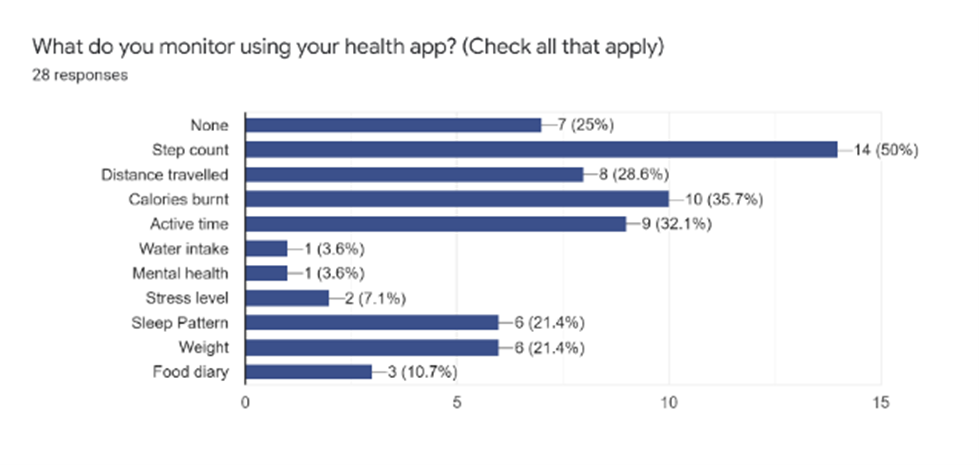
\includegraphics[width=\linewidth]{dissertation/images/2.png}
  \caption{Top Features Monitored}
  \label{fig:sub1}
\end{subfigure}%
\begin{subfigure}{.5\textwidth}
  \centering
  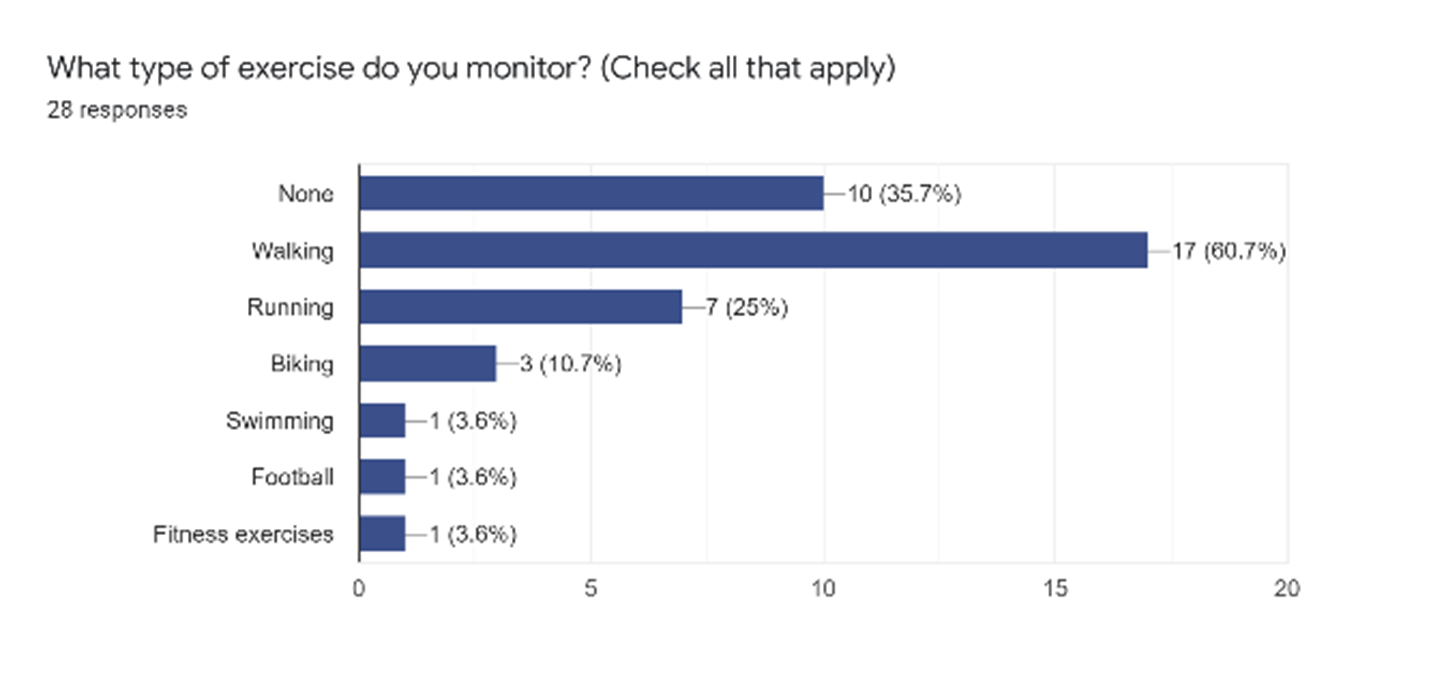
\includegraphics[width=\linewidth]{dissertation/images/1.png}
  \caption{Top Forms of Exercise}
  \label{fig:sub2}
\end{subfigure}
\caption{A Initial questionnaire to gather requirements}
\label{fig:test}
\end{figure}

 
\section{Initial Questionnaire  }
To identify the functional and non-functional requirements of this project, an initial questionnaire \ref{Appendix A} was designed to see what current features stakeholders would want to see in a step tracking game. Thirty participants completed the survey, all between the ages of 19 to 34 years old, with varying experience with fitness trackers. The questions comprised what effect of the COVID-19 pandemic on their mental and physical health, if they use fitness trackers, what features they would want to see in the application and their first thoughts on the game concept. The results of the effect of the COVID-19 pandemic are discussed further in chapter 6. 

\vskip 0.5em
Participants were asked what features they commonly used in fitness trackers, if they used fitness trackers, shown in \textbf{Figure 3.1 (a)}. The top three features were step count, calorie counter, and distance traveled. In the questionnaire, the most common monitored forms of exercise can be seen in \textbf{Figure 3.1 (b)}. The top form of exercise was walking, which supported the findings of the Active 10 paper, which found walking was the most common form of exercise in the UK. The feature suggestions, ranged from user customization, having a mini-game within the team, and being able to select the activity levels. A notable reply to the feature suggestion question was: \vskip 0.5em

\emph {“Involving team in collective and personal challenges, inclusive teams and challenges for all activity levels, prioritise exercise for mental and physical health without focusing too much on body weight (which is what annoys me the most in other fitness apps, the pressure to achieve the so called "goal weight").”}
\vskip 0.5em
This response from the participant encouraged me to not implement the second most used feature that the participants typically monitor in fitness trackers in order not to discourage any users from using the application. It solidified that the aim of the mobile application should be primarily to promote mental health through regular physical activity and be inclusive to all user groups whose levels of activity have been affected by the COVID-19 pandemic. It should not focus on calorie counting. 



\section{Functional \& Non-functional Requirements  }

Below are the documented requirements that were gathered from the project objectives, the background research as well as the requirements collected directly from the stakeholders. The requirements are split into two categories- functional and non-functional requirements. Non-functional requirements are attributes that the mobile application should have, such as usability or security. Functional requirements are what the system should do, such as user authentication or team creation. 
To prioritize the requirements accordingly, the MoSCow method [\citenum{27}] was used. For each iteration, the “must-have” requirements took priority in order to deliver a working prototype that was the minimum viable product. The “should have” requirements were also included in the sprint goals alongside these. If time allowed at the end of the sprint, the “should have” requirements were developed.
 
 \textbf{Must Have } These requirements comprise the minimum viable product and are essential for the end product to have, or it would not function properly.\vskip 0.5em
 \textbf{Should Have } These requirements are not essential for the system to function yet are still an important part of the system that would otherwise be missed by a stakeholder.\vskip 0.5em
  \textbf{Could Have } These requirements are desirable features that the project would benefit from if there is time for it at the end of a sprint. \vskip 0.5em
 \textbf{Would Like To Have } These are requirements that the project timeline does not allow for yet could be implemented in the future. 
 
 


% Please add the following required packages to your document preamble:
% \usepackage[table,xcdraw]{xcolor}
% If you use beamer only pass "xcolor=table" option, i.e. \documentclass[xcolor=table]{beamer}
\begin{table}[]
\begin{tabular}{lll}
\rowcolor[HTML]{FFFFFF} 
\multicolumn{1}{c}{\cellcolor[HTML]{FFFFFF}{\color[HTML]{000000} \textbf{Requirement}}}     & \multicolumn{1}{c}{\cellcolor[HTML]{FFFFFF}{\color[HTML]{000000} \textbf{Description}}}                                                                                                                                                                                                  & \multicolumn{1}{c}{\cellcolor[HTML]{FFFFFF}{\color[HTML]{000000} \textbf{Type}}} \\
\rowcolor[HTML]{9B9B9B} 
\multicolumn{1}{c}{\cellcolor[HTML]{9B9B9B}\textbf{}}                                       & \multicolumn{1}{c}{\cellcolor[HTML]{9B9B9B}\textbf{Must Have Requirements}}                                                                                                                                                                                                              & \multicolumn{1}{c}{\cellcolor[HTML]{9B9B9B}\textbf{}}                            \\
Activity Tracker                                                                            & \begin{tabular}[c]{@{}l@{}}The application has to track a person’s step count live and\\  the show daily total step count.\end{tabular}                                                                                                                                                  & Functional                                                                       \\
Team                                                                                        & \begin{tabular}[c]{@{}l@{}}To make a social collaborative mobile application  a user will\\  need to be part of a team.\end{tabular}                                                                                                                                                     & Functional                                                                       \\
Team Code                                                                                   & \begin{tabular}[c]{@{}l@{}}A user should be able to join a specific team they want using \\ a team code, join a random team or create their own team.\end{tabular}                                                                                                                       & Functional                                                                       \\
Team goal                                                                                   & \begin{tabular}[c]{@{}l@{}}A team must have a collective goal that they work towards \\ together and receive a form of reward. They will either win\\  and escape the zombies or they will lose, and their team \\ will be deleted. Focus on collaboration not competition.\end{tabular} & Functional                                                                       \\
Back-end                                                                                    & \begin{tabular}[c]{@{}l@{}}Back-end should be fast to implement. It should be secure,\\ dependable and have a quick response time.\end{tabular}                                                                                                                                          & Non-Functional                                                                   \\
\rowcolor[HTML]{C0C0C0} 
                                                                                            & \multicolumn{1}{c}{\cellcolor[HTML]{C0C0C0}\textbf{Should Have Requirements}}                                                                                                                                                                                                            &                                                                                  \\
Goal Setting                                                                                & \begin{tabular}[c]{@{}l@{}}Allow individual to specify their own different activity levels\\  goal rather than having one standard goal for everybody.\end{tabular}                                                                                                                      & Functional                                                                       \\
\begin{tabular}[c]{@{}l@{}}Track other team\\  member’s activity\end{tabular}               & Get live summary of teams weekly and daily step count.                                                                                                                                                                                                                                   & Functional                                                                       \\
\begin{tabular}[c]{@{}l@{}}Two player \\ competitive \\ game\end{tabular}                   & \begin{tabular}[c]{@{}l@{}}Implement a one-on-one, 10 minute mini game within the team \\ to add a social/competitive aspect that can be played  when   \\ user ready.\end{tabular}                                                                                                      & Functional                                                                       \\
\begin{tabular}[c]{@{}l@{}}Visualisation of \\ individuals physical\\ activity\end{tabular} & \begin{tabular}[c]{@{}l@{}}Get aggregated weekly data of an individual’s physical activity \\ and display on graph.\end{tabular}                                                                                                                                                         & Functional                                                                       \\
User Profile Picture                                                                        & \begin{tabular}[c]{@{}l@{}}Allow a user to personalize their account and be identifiable \\ within their team.\end{tabular}                                                                                                                                                              & Functional                                                                       \\
User Experience                                                                             & Ensure good user experience through a simple, consistent design.                                                                                                                                                                                                                         & Non-Functional                                                                   \\
Usability                                                                                   & \begin{tabular}[c]{@{}l@{}}Evaluate the usability. Follow usability heuristics to ensure\\  mobile application is usable.\end{tabular}                                                                                                                                                   & Non-Functional                                                                   \\
\begin{tabular}[c]{@{}l@{}}Automatically\\ track fitness data\end{tabular}                  & \begin{tabular}[c]{@{}l@{}}The tracker should not have to be manually recorded  by a  user, \\ instead step count should automatically be tracked.\end{tabular}                                                                                                                          & Functional                                                                       \\
\begin{tabular}[c]{@{}l@{}}Get normalized \\ data of team\end{tabular}                      & Get the daily average step count of the team.                                                                                                                                                                                                                                            & Functional                                                                       \\
Mental wellbeing                                                                            & \begin{tabular}[c]{@{}l@{}}Gather data on mental wellbeing before and after pandemic \\ and compare mental wellbeing during app evaluation.\end{tabular}                                                                                                                                 & Non-functional                                                                   \\
Game Narrative                                                                              & \begin{tabular}[c]{@{}l@{}}To make a gamified mobile application it must have an \\ underlying engaging storyline of zombies with a corresponding\\  user interface   to go along with it.\end{tabular}                                                                                  & Non-Functional                                                                   \\
\rowcolor[HTML]{9B9B9B} 
                                                                                            & \multicolumn{1}{c}{\cellcolor[HTML]{9B9B9B}Could Have Requirements}                                                                                                                                                                                                                      &                                                                                  \\
\begin{tabular}[c]{@{}l@{}}Track distance\\  travelled\end{tabular}                         & \begin{tabular}[c]{@{}l@{}}Get and display the live distance travelled alongside step count\\  data.\end{tabular}                                                                                                                                                                        & Functional                                                                       \\
\begin{tabular}[c]{@{}l@{}}Differentiate between\\  physical activities\end{tabular}        & \begin{tabular}[c]{@{}l@{}}Track different aerobic exercises other than walking, such as brisk\\  walking or running.\end{tabular}                                                                                                                                                       & Functional                                                                       \\
Mood Tracker                                                                                & Integrate mood tracking to further promote mental health.                                                                                                                                                                                                                                & Functional                                                                       \\
Water tracker                                                                               & \begin{tabular}[c]{@{}l@{}}Promote physical health by adding a range of health activities\\  such as a water tracker.\end{tabular}                                                                                                                                                       & Functional                                                                       \\
Push Notifications                                                                          & \begin{tabular}[c]{@{}l@{}}Send reminder notifications to user to keep walking or notify \\ when time will run out.\end{tabular}                                                                                                                                                         & Functional                                                                       \\
\rowcolor[HTML]{9B9B9B} 
                                                                                            & \multicolumn{1}{c}{\cellcolor[HTML]{9B9B9B}\textbf{Would Like To Have}}                                                                                                                                                                                                                  &                                                                                  \\
Requirement                                                                                 & Description                                                                                                                                                                                                                                                                              & Type                                                                             \\
Companion Website                                                                           & \begin{tabular}[c]{@{}l@{}}Get a partner side to accompany to application, where team \\ members can communicate with each other and interact with \\ other teams.\end{tabular}                                                                                                          & Functional                                                                       \\
Publish on Test Flight                                                                      & \begin{tabular}[c]{@{}l@{}}Configure the application for iOS devices using XCode. Once\\  configured, let people evaluate it by publishing it on test flight.\end{tabular}                                                                                                               & Functional                                                                       \\
Publish on Google Play                                                                      & \begin{tabular}[c]{@{}l@{}}Once application tested it can be published on the Google play\\  store.\end{tabular}                                                                                                                                                                         & Functional                                                                      
\end{tabular}
\end{table}









 
 
\chapter{Design }

\section{Iterative Model}
  \begin{figure}[h]
    \centering
     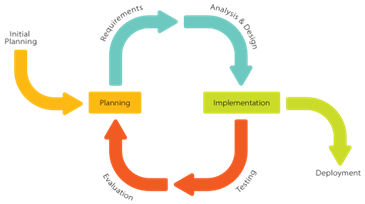
\includegraphics[width=90mm]{dissertation/images/3.png}
     \caption{Iterative model}
     \setlength{\belowcaptionskip}{-10pt}
     \label{fig: Forms of exercise}
 \end{figure}
At the start of week four of the project, I employed an iterative approach [\citenum{28}] and split the project into ten separate sprints, each lasting the standard length of two weeks. The model can be seen in \textbf{Figure 4.1}.
 Breaking down the project into smaller sections made the objectives manageable, and with each cycle, I was able to produce a refined version of the product until a final version was accomplished. At each stage, objectives were set out, implemented, tested, and reviewed. Deployment to stakeholders occurred less frequently- only when the prototype and final product were being evaluated did the versions get deployed.
At the start of each iteration, I set out the goals for the sprint by looking at my requirements and taking into account what was achieved in the previous sprint—using this, if any goals were not met from the previous sprint, they would be achieved in the coming sprint. By following this method, features were added in increments to achieve the final product. 



\section{System architecture}

  \begin{figure}[h]
    \centering
     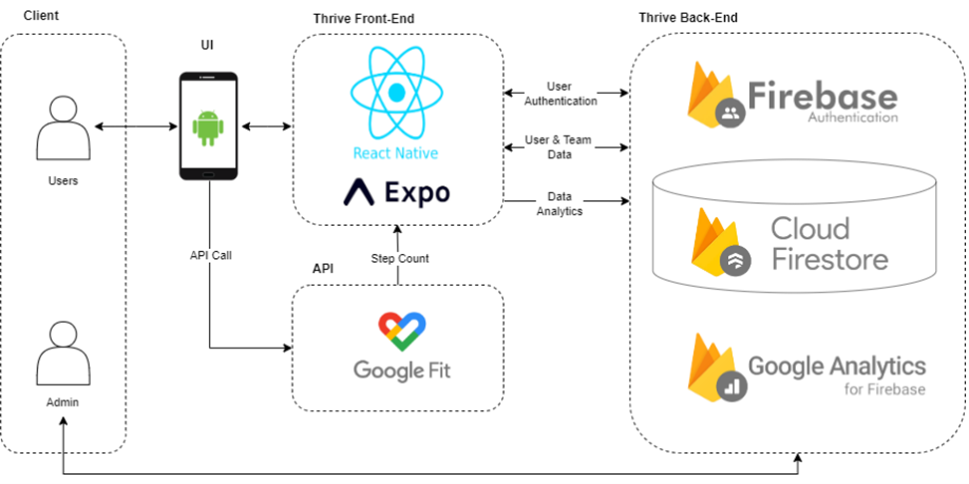
\includegraphics[width=95mm]{dissertation/images/4.png}
     \caption{Initial System Architecture}
     \setlength{\belowcaptionskip}{-10pt}
     \label{fig: Forms of exercise}
 \end{figure}

To design the initial system architecture of the mobile application, different frameworks and services were considered. The research was conducted to decide on the three important aspects of the application- front-end, back-end, and considering how to gather the step count of a user. The initial system architecture designed at the start of the project can be seen in \textbf{Figure 4.1}. \vskip 0.5em
For the front-end of the application, React Native was chosen alongside Expo. Originally, for the back-end, I chose to use Amazon Web Services, which was later replaced by Google Firebase due to it being more beginner-friendly in comparison. Firebase has more readily available resources and tutorials, whilst AWS offers a wide range of services (over 200 services) with less extensive resources. Firebase is suitable for small-scale projects and is a real-time database that offers low latency. \vskip 0.5em
 To gather physical activity data, I researched different methods to get the data for react-native. Accelerometers, pedometers, and other services were considered. An important requirement for the activity tracker was that a user should not have to manually record their own steps. This would be needlessly inconvenient and affect the usability of the application. Google Fit met the requirements of gathering the data automatically without the need for a user to record their own steps. It is a popular package and is widely used by other mobile applications. It offers a range of health data that can be tracked, such as weekly and daily step count, distance traveled, duration of a workout, hydration, as well as differentiating between different exercises. These were all features I was interested in implementing for the project. 
 

  \begin{figure}[h]
    \centering
     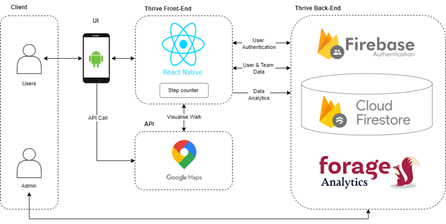
\includegraphics[width=95mm]{dissertation/images/5.png}
     \caption{Final System Architecture}
     \setlength{\belowcaptionskip}{-10pt}
     \label{fig: Forms of exercise}
 \end{figure}
 
The final system architecture diagram can be seen in \textbf{Figure 4.1}. The earliest change made to the architecture was to discard Expo so as to reduce the size of the application. Another benefit gained with using bare react-native was that it does not restrict the project to Expo-only libraries, which would have affected the development speed of the application in future iterations. \vskip 0.5em
There were several issues with using Google Fit to collect the user step count data throughout the iterations. When the team challenge feature was implemented, the step data could no longer simply be read but had to be written to. The API did not support this, and a different solution had to be used. I chose to use a React Native library that made use of the phone's inbuilt sensors to get the step count and allowed for step data to be updated. \vskip 0.5em
Lastly, to analyze data from testers, Google Analytics was used to create custom events to gather data from specific events made by a user. However, there was an issue getting the custom parameters, and the custom events could not be seen. This was solved by using Forage- an analytics tool explicitly made for React Native applications. 

\section{UML Use-case diagram}


  \begin{figure}[h]
    \centering
     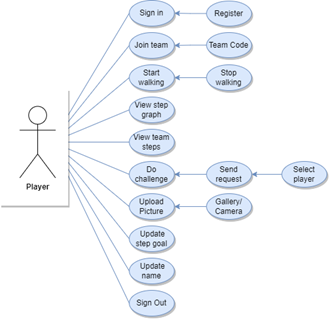
\includegraphics[width=50mm]{dissertation/images/6.png}
     \caption{UML diagram}
     \setlength{\belowcaptionskip}{-10pt}
     \label{fig: Forms of exercise}
 \end{figure}
 
A unified modeling language (UML) use-case diagram identifies the different interactions that different types of users should be able to perform with a system. It is a high-level way to describe the requirements of a system. This was used during the requirements gathering phase to understand what had to be implemented. In the mobile application, there exists only one actor, and that is a player. A player will interact with the mobile fitness tracker application, as seen in \textbf{Figure 4.4}. 

\section{Technology}

This subsection discusses the coding tools that were used to design the mobile application.  \vskip 0.5em
 \textbf{Android} \vskip 0.5em
I chose to develop the mobile application for Android devices as I had readily available access to an Android device. Developing for Android, as opposed to iOS, is less restrictive due to the lower cost of development. However, it takes longer to develop and is considered more complex due to how varied Android devices are. \vskip 0.5em
 \textbf{React Native} \vskip 0.5em
React Native uses JavaScript to develop cross-platform applications for Android and iOS mobile devices. It offers a range of libraries due to its strong community, reduces the time to develop, and is beginner-friendly. I chose to use the software framework React Native to develop the application for Android. The reason I chose it was due to how popular the framework was, with companies such as Instagram and Meta using it to create their applications. \vskip 0.5em
 \textbf{Firebase}\vskip 0.5em
I considered using AWS Amplify for the back-end however switched to Firebase during later iterations due to how little documentation there was for developing React Native apps with AWS. Firebase is a beginner SDK friendly to the setup requiring minimal steps while offering valuable services such as authentication and analytics services. It is a NoSQL database, meaning data is not confined to a set structure as opposed to a nonrelational database that stores data in rows and columns. Being a serverless framework, it reduces the time to develop mobile applications significantly, which is appropriate for a small project.\vskip 0.5em
 \textbf{Forage Analytics} \vskip 0.5em
Forage Analytics was utilized to design custom events on top of the standard custom events Google Analytics offers. Unlike Google Analytics, Forage is designed specifically for React Native applications. This is an advantage as I experienced difficulty accessing the data of the custom events I had created on Google Analytics. It allowed me to gather specific data, such as when and how many steps a participant had done during the user study.\vskip 0.5em
 \textbf{Google Maps}\vskip 0.5em
Google Maps is a feature most consumers are familiar with, especially when using fitness trackers. It is a natural step to extend the functionality of the mobile application and is usually pre-installed onto devices. A drawback to using Google Maps is that it is necessary for users to have access to a network connection to access their location. 

\section{Iterations}

The following subsection will outline the modifications made throughout the ten different iterations. 

\subsection{Iteration 1}



  \begin{figure}[h]
    \centering
     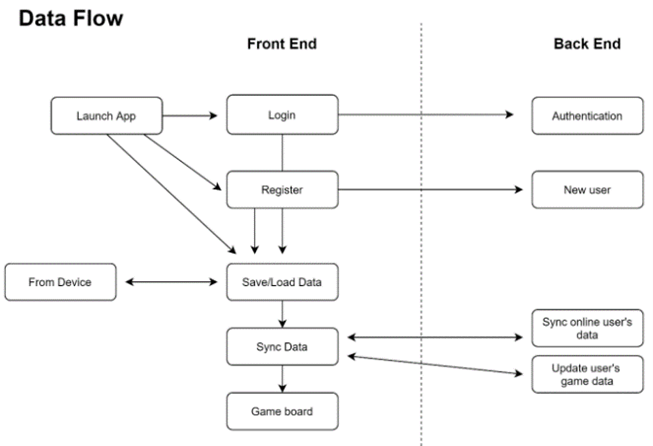
\includegraphics[width=70mm]{dissertation/images/7.png}
     \caption{Data Flow Diagram }
     \setlength{\belowcaptionskip}{-10pt}
     \label{fig: Forms of exercise}
 \end{figure}
 
Prior to the first iteration, I reviewed different mobile applications to decide what this mobile application would focus on. The initial game idea was that it would revolve around zombies and a survival team to make it a collaborative game. 
The main objective for the first iteration was to get familiar with the app development frameworks that I would choose for the project. Moreover, I had to start designing paper prototypes of the initial user interface. \vskip 0.5em
After considering different frameworks, I selected React Native, Expo, and AWS to implement the application and started learning app development with React Native. I chose React Native over Flutter due to its prevalence, stronger community, and range of libraries. The framework Expo was used because it is recommended when you want to develop an application rapidly. For the back-end, I chose AWS because they offer a fast number of services. I created a system architecture diagram and data flow diagram (\textbf{Figure 4.5}) to help start setting up the back-end.   \vskip 0.5em
I continued researching different mobile fitness trackers throughout this iteration to refine the game concept and design the UI. For my dissertation topic, I decided to focus on the pandemic's impact on physical activity and mental well-being. To gather data on this topic, I sent out a survey to see if it was a viable topic, what features to include in the app and initial thoughts from the stakeholders. 
The initial user interface had four screens- the main page to show a map that the user progresses through; a character page to view the different team members on the team; a statistics page view for a user to view data such as calories burned and total active time and an achievements page. A paper sketch of the screens can be seen in \textbf{Figure 4.6.}. \vskip 0.5em

  \begin{figure}[h]
    \centering
     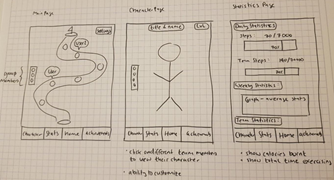
\includegraphics[width=70mm]{dissertation/images/8.png}
     \caption{Initial Sketch}
     \setlength{\belowcaptionskip}{-10pt}
     \label{fig: Forms of exercise}
 \end{figure}
 
The game concept was inspired by Minecraft's survival mode and Zombie, Run!. The mobile application Thrive is a step tracking game that lets you play with your friends as you try to survive and thrive in a zombie apocalypse world. The purpose of the game is to combine a social aspect with trying to encourage consistent daily activity in an individual. A user will find teammates to explore a town with and scavenge for resources to upgrade and rebuild their shelter. During the daytime, each teammate will explore the town alone to collect resources that can be used for the teams' shelter and to customize a user's character. The team will take shelter during the nighttime while the zombies destroy their group shelter. The fewer steps a team has made, the more damage the zombies will make. If the zombies damage the shelter enough, it will fail, and the game will end.\vskip 0.5em

Main features:\vskip 0.5em
\begin{itemize}
\item Survival log: Players can view their own and their teammate's fitness activity
\item Unlock achievements: Players can unlock team and individual achievements 
\item Collaborative aspect: The more resources a team collects, the higher the chances of survival
\item Challenge teammates: A user can challenge a teammate to other health-related tasks such as: meditating, drinking a glass of water, eating a piece of fruit, etc.
\item Time limit:  The team has until nighttime to collect resources
\item Leader board:  A player can view their ranking within the team to promote competition and motivation
\end{itemize}
At the end of the iteration, I evaluated that I had met the objectives for the sprint by choosing the frameworks and started learning about them. From carrying out background research, I had found a topic for the dissertation and would focus my research on it. For the next iteration, I had to start thinking about sending data to and from with AWS Amplify.   


\subsection{Iterations 2}
From the review of iteration 1, I had to focus on passing data to the back-end with React Native and AWS. Unfortunately, during this iteration, I had a family emergency, and the goal for this iteration was moved to iteration 3. 


\subsection{Iterations 3}
The goals for this iteration were to consider how to get the step data from the user and to continue working with React Native and AWS. 
For the back-end, I chose to move away from AWS and use Firebase instead after not making progress with it. I found Firebase better to work with due to it being beginner-friendly and not needing other services or having to provide payment details. It was easier to understand and had resources readily available. \vskip 0.5em
During the iteration, I followed along with a course on React Native and Firebase to implement a restaurant application. After looking at different React Native packages and APIs, I chose to use Google Fit API as it could manually record the steps of a user and met the requirements of collecting daily and weekly step count data. From reviewing the survey response, I found that there was a positive response to my game concept. \vskip 0.5em
By the end of this iteration, I had started using Firebase with React Native and had chosen how to collect the step count that met the criteria. The system architecture diagram can be seen in \textbf{Figure 4.2}. Moving forward, I needed to get the step count from a player. 
\subsection{Iterations 4}
The goals for this iteration were to implement the step counter, set up four basic screens, implement the login screen and start working on the team joining functionality. 
I set up the project on Firebase to start using its authentication service. Users should log in or register to the app, and then see four different blank pages. The four pages will be the user activity, team activity, map, and challenge page. To implement the join a team function, the user collection would need to store the team code, and the teams collection would store the details of four players- email and a unique ID. On the activity page where it should show the step count, there was an issue that meant the step count was not displayed. Testing was done using the emulator and debugging using console.log. 
At the end of iteration 4, I had the login and register feature working; this page led to four blank pages using a bottom tab navigator. I started designing the data structure of the teams and users collection on paper for the join a team functionality. I ran into trouble with the step counter not giving data. Moving forward, the step counter and team functionality goals would have to be shifted to iteration 5. I also began thinking about the long-term goals for the next iterations. I had to work towards having a minimum viable product that could be deployed and evaluated by participants. This would mean revising the main features from iteration 1. 

Goals for semester two: 
\begin{itemize}
\item Have a working prototype ready to test with users
\item Decide how many users to test application
\item Let users chose their own fitness level
\item Do background research to investigate the effect of fitness application on mental wellbeing
\end{itemize}

\subsection{Iterations 5}
  \begin{figure}[h]
    \centering
     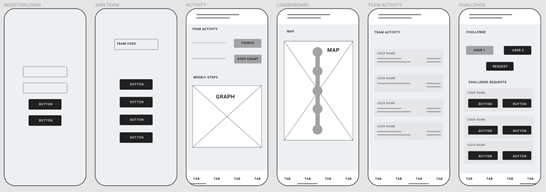
\includegraphics[width=110mm]{dissertation/images/9.png}
     \caption{MVP Wireframes}
     \setlength{\belowcaptionskip}{-10pt}
     \label{fig: Forms of exercise}
 \end{figure}
 
The main goals for this iteration were to refine the main features for the minimum viable product; fix the issue with the step count, and implement the join a team feature. 
The minimum viable product (MVP) would be six screens: login/register, join a team, user activity, map/leader board, team activity, and challenge screen. The activity page would display the step count, points, and graph. The leader board screen would display the team players' names and where they were on the map. The activity page would show the player's step count and points. Players can select another player and send them a challenge to complete on the challenge page. \textbf{Figure 4.7} shows the Figma wireframe for the MVP.  
During this iteration, I restructured the project to not use Expo. Using Expo took up a lot of storage space for a small number of screens. By the time I had produced the prototype, it would be too bulky. To run the application on my device without using Expo, I enabled debugging on my device. Running the application on my device meant I could test if the different features worked as features were added. A top tab was added to display the date. I used the database structure from the previous iteration to implement the users and teams collection. For the join a team feature, users should have three ways to join: they can join a random team, create a team by specifying their team code or join by inputting a team code. Additionally, they had the option to sign out. The previous issue with Google Fit was that a user could not approve the application to access the step count data, so the Android permissions were added. 
At the end of iteration 5, I refined what features should be included in the prototype by removing any unnecessary features from iteration 1 and including the should have features. Using this, I designed the wireframes for the screen to make it clear what to create for the next iterations. Going forward, I need to ask a player permission to access their step count and complete the activity page functionalities. 

\subsection{Iterations 6}
The goals for this iteration were to request permission to get the step count from Android; finish the join a team page; display the step count, and add a graph to the activity page.\vskip 0.5em
To get the step count data, a user had to grant permission, and if so, they were then prompted to log in through a Google account to access their step data. This was then displayed on the activity page, and a bar chart plotted the step count for the week. The experience points a user can collect were also derived from a player's steps. To identify players and display their names throughout the app (such as along the map), I added another input option on the join a team page. The username, today's total steps, and weekly steps object (containing data on each walking session) is sent to the users collected. For the join, a team page, the team collection stored the unique team code, and an object called members to store the details (email and unique user ID of the user) of the four-team members. 
Create a team option: a new team was made using the unique team code specified by the user inside the team's collection on Firestore, and the user was listed as a member of that team. Team codes have a maximum length of 5 integers for ease of use. Join a team option: the unique ID and email of the user were added to the member's object of the team's collection. Join a random team: if the team code exists in the team's collection, the user was added as a team member. For the map screen, the username of players was displayed according to their step count, along with a step indicator. The step indicator has six steps that represent zero to five thousand steps. To test the new features added, I created an APK. This allowed me to see if the functionality was correct by creating a four-player team. By walking as the team members, I was able to see if the map progression feature worked correctly. \vskip 0.5em
The objectives for the iteration were met. The results from the test walk revealed that players moved along the step indicator correctly; however, some refinements needed to be made to the two pages. For the find a team page, if a user created a team using an existing team code, they would join that team even if it was full of four players. I fixed this by making the member's object have a max length of 4 and alerting that the team code already exists. Lastly, if a username was too long, it would not display correctly. Going forward, I had to continue working on the map page and start on the activity page that displays the physical activity of the other team members. 
\subsection{Iterations 7}
The goals for this iteration were to display the team data on the activity page, implement the challenge function and resolve the issues from the last iteration. Once these features were completed, it would make up the minimum viable product that contains all the "should" functional requirements. A key goal for this iteration should be to get stakeholders to give feedback about the minimum viable product. 
The username was restricted to 5 characters during this iteration to correct text overflow on the activity page. When users tried to join a full team, they received an alert dialog informing them that it already existed. The username was given a bubble on the map screen to make it clear that it represents one user and does not overlap. The player's physical data was retrieved and displayed on the team activity page from the team collection. Team players were displayed in order of step count. 
The UI of the challenge screen was created. A modal showed the team members' names for the challenge feature that a user could select and send a challenge request. The team member then accepted the challenge, which sent them to a new page displaying a countdown and the step count. The steps are sent to the user collection when the timer is over. If a user declines or is completed, the challenge request disappears from the UI. A challenge object was created in the user's collection; each request sent had a unique ID. If the request was declined, it was removed using its unique request ID. It specified who the challenger and the challenged player were. 
 The demonstration of the MVP was done over zoom with six stakeholders. 
 
 \vskip 0.5em Here are the critical comments made about the app: 
\begin{itemize}
\item Improve the challenge feature by not letting the player who sends the request to participate in the challenge- having two players battle each other makes the game competitive and engaging 
\item The theme of zombies was engaging but was unclear in the game
\item The bar chart did not convey the changes in step count correctly,  replace with a line graph so changes can be tracked over time
\item Needing to install Google Fit to use the application was inconvenient, and you could check your steps on Google Fit instead
\item Improve the design by adding more images and color 
\item Instead of having usernames represent the players on the map, they should be represented by a character 
\item Display the team code on the team activity page, so a player does not forget what team they belong to
\item Having one page to log in and register is uncommon and should be split into two separate pages
\end{itemize}

Following the feedback, I added a settings page where a user could upload a profile picture and update their username. The profile picture was added to the challenge screen when a user selected a user from the modal. 

By the end of the iteration, the team activity and user page were completed meaning the MVP was achieved. I conducted a demonstration of the MVP prototype to the stakeholders and received feedback to improve the product to create a prototype that participants in the next iteration can evaluate. 


\subsection{Iterations 8}
The main goal for this iteration was to give a large number of participants the prototype so they could run it on their devices. Additionally, the features suggested in the demo by participants should be implemented.  
The bar chart package was replaced with a liner chart graph to help users visualize the change. An APK was then given out to 10 participants for one day. This evaluation aimed to identify any bugs with the app before conducting the final evaluation and further gathering feedback to refine the prototype. 

\vskip 0.5em Feedback/Issues reported: 
\begin{itemize}
\item Nearly all users reported the app crashing when trying to register or login multiple times
\item App froze for a few seconds when joining a team
\item The graph was cut off- the date was not able to be seen
\item The user's profile picture did not display on the challenge page
\item Design feedback: add images, colors, and an app icon 
\item Add a page to see details of past challenges
\item Add a feature to invite friends to join the team a player is in 
\end{itemize}
\vskip 0.5em 
I added a feature to check if the team had achieved the daily goal. If they had- a modal would notify them, and if they lost, their team would get deleted. I refined the challenge timer by allowing the timer to run in the background without stopping. I found out that the application crashing was due to errors not being handled properly with trying to register/log in. This was fixed, and then the page was split into two separate components to follow conventions. Furthermore, the challenge feature was improved to allow two players to partake in the challenge. A past challenge screen was added to view the details of the past challenge and let users see who had won or lost the challenge. 
By the end of the iteration, the prototype was tested by users and identified critical bugs and, supported the feedback given by the ten participants, reflected the demonstration feedback from the three participants. By the end of the iteration, I identified critical bugs that were resolved and more features to be implemented before the final user evaluation. For the following iteration, I decided to gather analytic data to supplement the final evaluation to check the authenticity of feedback from participants.  

\subsection{Iterations 9}
The goals for this iteration were to increase the product's attractiveness, design the final evaluation, and gather analytic data. 

  \begin{figure}[h]
    \centering
     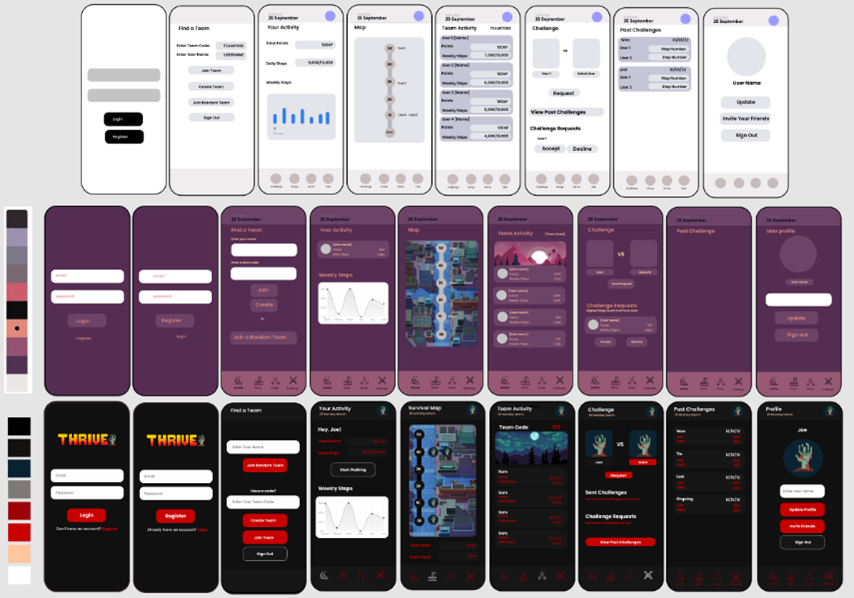
\includegraphics[width=90mm]{dissertation/images/10.png}
     \caption{UI Designs}
     \setlength{\belowcaptionskip}{-10pt}
     \label{fig: Forms of exercise}
 \end{figure}

During the iteration, the final overall look was decided. To fit the theme of zombies, a dark color scheme was chosen over a light color scheme, and related images were added through the UI. A splash screen was added, and custom modals were created to follow the app's overall look. 
User experience was enhanced by adding an animated loader to give feedback that the application is not frozen and is retrieving information from the back-end. The UX was improved further by using custom modals to provide feedback to the user about changes made in the app, such as informing the user the challenge is up. The evolution of the UI can be seen in \textbf{Figure 4.8}. The profile pictures were added to the map page instead of displaying the player's name; custom fond was added; intro slides and the bottom tab highlighted what page a user was in by displaying active/inactive icons. The introduction slides would contain a health warning, the story behind the game, and fitness advice to inform a user how much to walk. 
To gather analytic data, Google Analytics was used to send data on custom events that a user performed. There was an issue with the custom parameters returning empty to Firebase. After trying to fix this issue and following documentation on tracking custom events, I still could not retrieve the data. 
During this iteration, I checked the application's functionality and noticed that the challenge steps were not being added to the Google Fit step data. This was an issue as the step count should reflect all the user's physical activity; if not, a user would not feel compelled to take part in the mini-challenges. Due to this, I chose to use the step counter package considered in the earlier iterations. This would need that the step counter would no longer automatically track a user's physical data. However, it would mean that a user did not have to download Google Fit on their device. A user timer page was added, similar to the challenge timer. 
By the end of the iteration, the application's UI had been improved, and I was able to get feedback on the evaluation plan. A different step counter was used. For the following iteration, I had to look at using different analytic tools and focusing on the final product. 

\subsection{Iterations 10}
The main goals for the last iteration were to choose a different analytics tool, review what requirements have not been met, and conduct the evaluation. 
During this iteration, I reviewed what requirements had not been met. This led me to add a feature where users could select their daily fitness goal- ranging from 1 to 10 thousand steps. The survival log modal was fixed to display daily when a user logins. Forage was chosen over segment as it was specifically made for React Native applications, and I was able to get the custom parameters. In the remaining time I had left, I added Google maps to the walking pages so users could visualize their walk and added the kilometers walked. 
For the final user evaluation, the study guide was finalized and given to 8 participants given the APK to test within their team. 

\chapter{Implementation }

  \begin{figure}[h]
    \centering
     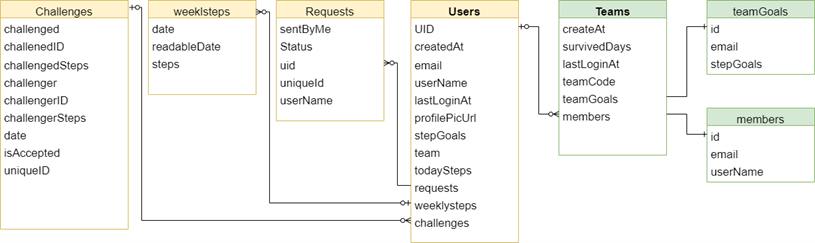
\includegraphics[width=140mm]{dissertation/images/12.png}
     \caption{Database Schema}
     \setlength{\belowcaptionskip}{-10pt}
     \label{fig: Forms of exercise}
 \end{figure}
 
\section{Back-end}
This chapter discusses the specifications of the main features of the mobile application. The final application can be found in the GitHub repository \ref{Appendix D}. 
The Firestore real-time database contains two collections called users and teams for the application. Within these collections, data is stored in the documents for each player and team. \textbf{Figure 5.1} depicts the structure of the final Firestore database using an entity-relationship diagram. A user can be part of many or no teams, and a team contains at least one user. The team's collection contains information on each team member who is part of the team, such as their name, step goal, and the days the team has survived. The user's collection stores their profile picture, challenge requests they have sent, the number of steps they did during a challenge, and details on each walking session recorded. 

\begin{figure}
\centering
\begin{subfigure}{.50\textwidth}
  \centering
  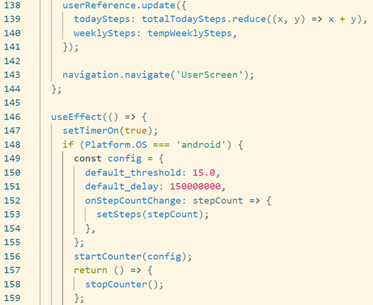
\includegraphics[width=80mm]{dissertation/images/13.png}
  \caption{Step Counter}
  \label{fig:sub1}
\end{subfigure}%
\begin{subfigure}{.5\textwidth}
  \centering
  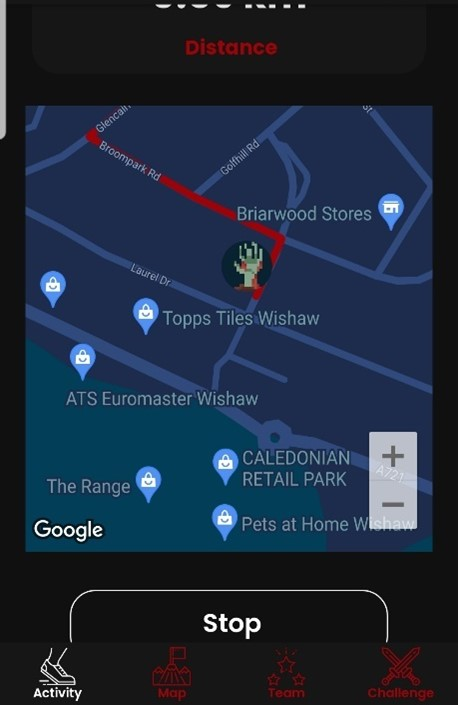
\includegraphics[width=40mm]{dissertation/images/14.jpg}
  \caption{Google Maps}
  \label{fig:sub2}
\end{subfigure}
\caption{Activity Screen Functionality}
\label{fig:test}
\end{figure}

\section{Step Tracking Functionality}
The application starts tracking the steps of a player when they manually record a walking session. Once a player presses "start walking," they are led to a different screen that starts a timer and records their steps. The user timer screen displays: the duration of the walk, step count, distance walked, and the walking route. Lastly, a player will stop their session, and they will be returned to the activity page. The step tracker is rendered inside the userTimer screen, and the finishChallenge function updates the user collection. 
The steps data is collected using a React Native library called accurate step counter, as seen in \textbf{Figure 5.2 (a)}, lines 146-159. The step counter accesses a device's inbuilt sensors to detect the motion of a user. It outlines a threshold to determine what counts as a step and specifies the time between steps. The threshold value determines how sensitive a sensor will be. 
As seen in \textbf{Figure 5.2 (b)}, Google Maps is integrated into the application to let players visualize their walking route as they walk. A player must enable the location permission to display their location on the map. To get the distance walked by a player, the function calcDistance uses the haversine formula to calculate the difference between the new and old coordinates. The styling of the map was customized to match the color scheme. No data relating to a player's route is sent to the Firestore or stored.  
After a walking session, the player will press the stop button, and the finishChallenge function is called. This asynchronous function fetches data from Firestore using async and await. In this case, data is retrieved from the document matching the user's unique ID inside the user's collection. Await is used to temporarily pause the execution of an asynchronous function to wait for a different promise to be returned. Data containing the details of a walking session (tempWeeklySteps) and the daily step count (totalTodaySteps) is sent to a particular user's document, as seen in \textbf{Figure 5.2 (a)}. The data held inside the tempWeeklySteps is the number of steps data from the step counter, a date, and a readable date (used to display the line graph). The totalTodaySteps is a list that holds all the steps recorded for today's date. The list of steps is retrieved from tempWeeklySteps, by only selecting the step data that matches today's date. 


\section{Challenge Players}
A player can view the challenge request they have received or sent themselves on the challenges page. They can decline, accept or request to challenge a player. A user can decline a challenge sent to them by a team member. This is done by accessing the array of objects that holds data regarding challenges in Firestore. The function rejectChallenge tried to find the request identifier in the user challenge data. If it is found, challenge data is filtered using the unique identifier of the challenge request to exclude that specific challenge, and this new temporary array is used to update the player's challenge data. By doing this, a user can not take part in the challenge since it no longer exists in their document. A user requests a challenge from a player using the function sendRequest. This creates two new objects containing (tempRequest and tempChallenges) that will be pushed to the database. The request object specifies who sent the request, and the challenge object will hold the data about the challenge, such as the step count of the two users. They are used to specify who won or lost on the past challenges page. When players accept a challenge, they are led to a similar page like the timer screen. The only difference to this screen is that the duration of a challenge is set to 10 minutes. 

\section{Survival Log Feature}
\begin{figure}
\centering
\begin{subfigure}{.50\textwidth}
  \centering
  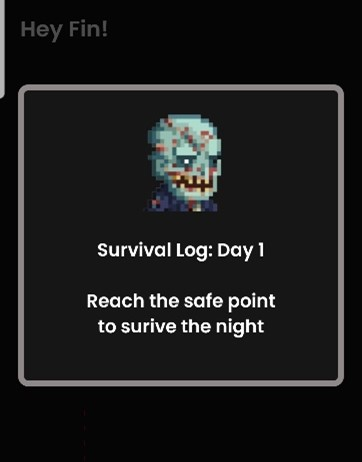
\includegraphics[width=40mm]{dissertation/images/15.jpg}
  \caption{Won Modal}
  \label{fig:sub1}
\end{subfigure}%
\begin{subfigure}{.5\textwidth}
  \centering
  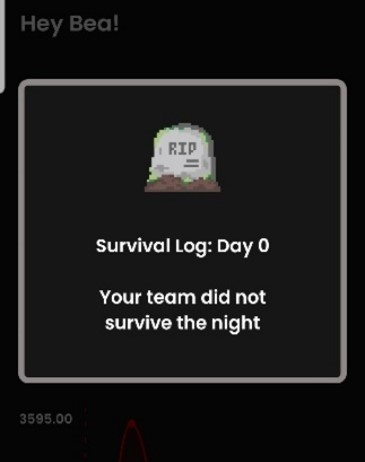
\includegraphics[width=41mm]{dissertation/images/16.jpg}
  \caption{Lost Modal}
  \label{fig:sub2}
\end{subfigure}
\caption{A Initial questionnaire to gather requirements}
\label{fig:test}
\end{figure}


The survival log acts as a daily reward by notifying a player if their team had survived the previous night and returned how many days they had survived. A player's team does not survive the night if they do not achieve their team goal. The team goal is the sum of the player's daily fitness goals. This ranges from 1,000 to 10,000 steps. The survival log feature is implemented using two main functions: checkTeamSteps and checkLogSurvivalDate.
The checkTeamSteps functional gets the todaySteps of every player that belongs to the team from the user collection. This gives the total steps done by every player and stores it inside checkSteps. The checkLogSurvivalDate function then checks when the team's last login date was. If the last login date was today, then the daily challenge is still ongoing and does not need to be checked. If the last login was not today, then the daily challenge needs to be checked. 
To see if the user achieved the daily challenge, the total stepGoals of every player in the team are retrieved from Firestore and are compared to the total steps in checkSteps. A team can continue playing the game when the total of stepGoals is less than the total steps. If the sum of the team's steps is greater, the team has achieved its collaborative goal and can continue playing. If the collaborative goal is not met, then the team has lost.
When a team wins, the survivedDays stored in the Teams collection will be updated by 1, and a modal will display how many days the team has survived so far. When a team loses, a modal will show how many days they survived and inform the player they have lost. Next, their team is deleted, and the player is pushed to the find team page to start a new game. A team is deleted by removing the team code from the user collection. 
This feature would typically be achieved using a back-end using a scheduled function. For example, it could have been implemented using Cloud Functions, a service provided by Firebase, and the survival-log function would be scheduled at midnight to check if the team survived. 


\section{Front-end}
I applied Stuart Pugh’s design methodology [\citenum{32}] of refining and discarding ideas during the iterations. This was done by sketching numerous ideas and moving on to designing detailed prototypes using Figma. To create a usable user interface, I ensured to follow the ten heuristics outlined by Jakob Nielsen [\citenum{31}]. For example, feedback on the system status was given to the user through modals and loading spinners to communicate that data was being retrieved or sent to Firestore. The final prototype, depicting all the screens and modals, can be seen in \ref{Appendix B}. Once this was done, users tested the interactive prototype to identify bugs and gather feedback about the application. This process kept repeating until the final mobile application was achieved. 


\chapter{Evaluation}


  \begin{figure}[h]
    \centering
     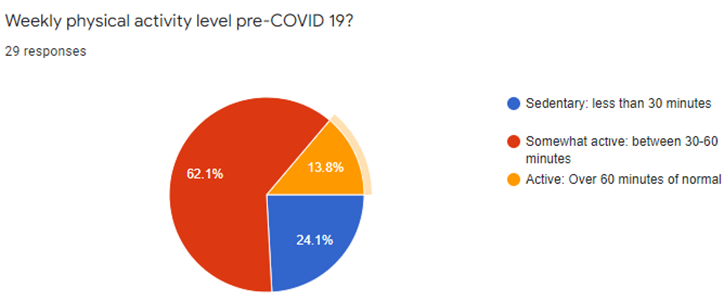
\includegraphics[width=90mm]{dissertation/images/17.png}
     \caption{Physical Activity Pre COVID-19}
     \setlength{\belowcaptionskip}{-10pt}
     \label{fig: Forms of exercise}
 \end{figure}
 
   \begin{figure}[h]
    \centering
     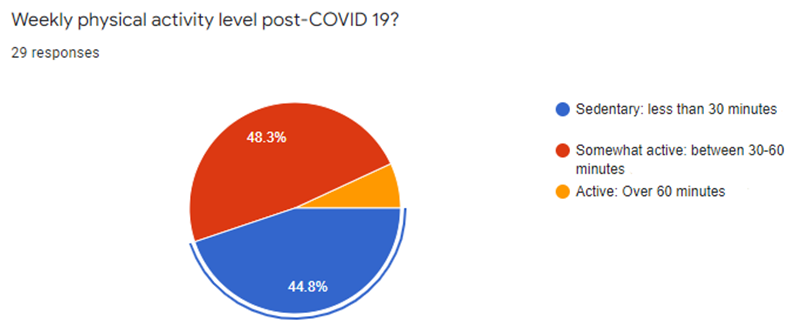
\includegraphics[width=90mm]{dissertation/images/18.png}
     \caption{Physical Activity Post COVID-19}
     \setlength{\belowcaptionskip}{-10pt}
     \label{fig: Forms of exercise}
 \end{figure}
 
\section{Initial Questionnaire Continued}
 This continues from section 3.1 and focuses on the mental and physical effect the pandemic has had on the participants. Twenty-nine participants between the ages of 19 and 35 took part in the survey, with one person being under the age of 18, thus was illegible to take part. The full anonymized results can be found in \ref{Appendix A}.

   \begin{figure}[h]
    \centering
     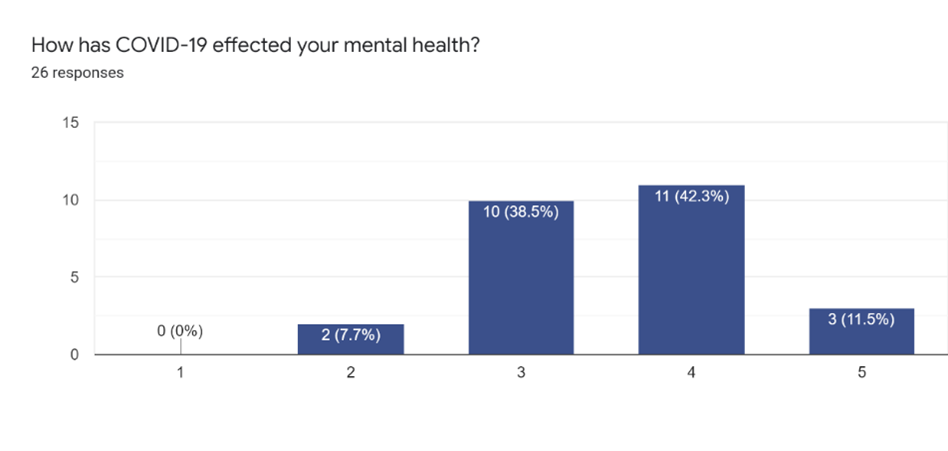
\includegraphics[width=100mm]{dissertation/images/19.png}
     \caption{Mental Health}
     \setlength{\belowcaptionskip}{-10pt}
     \label{fig: Forms of exercise}
 \end{figure}
 
 
 \textbf{Physical Activity }\vskip 0.5em
 Overall, before the pandemic, 76\% of participants followed NHS guidance of doing more than 30 minutes of weekly physical activity. After the COVID-19 pandemic, 54\% of participants followed the recommendation. The results reveal an increase of 20\% in sedentary behavior among adults.
 
\textbf{Mental Health }\vskip 0.5em
Overall, participants experienced a negative impact on their mental health due to the pandemic. Participants were asked what effect COVID-19 had on their mental health: 0\% noted a highly positive effect, 7\% noted a positive effect, 10\% noted a neutral effect, 42\% noted a negative effect, and 11\% noted a highly negative effect.



\section{Minimum Viable Product Demo \& Prototype}

During the start of iteration 7, an online demonstration of the minimum viable product, describing the game concept and its key features, was conducted to 6 relevant stakeholders over zoom. The MVP contained only the must-have elements outlined in the Requirements section. The demonstration was conducted to assess the first impressions of the mobile application and the acceptability of the different features. Notably, a participant commented that installing Google Fit made the application redundant. Overall, the app's first impression was positive, and no fundamental changes had to be made to the concept of the game. 
Following the positive reaction to the demonstration, the mobile application was tested by participants on their own devices. Ten participants and data carried out the initial evaluation of the prototype were gathered using a survey after they consented to take part in the short study \ref{Appendix C}. Participants carried out seven tasks to test all the different features on every screen and fill out the survey. The goals for testing the prototype were to identify any bugs and collect feedback on the functionality and design of the mobile application. Participants reported that the challenge functionality worked however it froze, it would stop responding briefly on the challenge page, and the application frequently crashed only when signing up or signing in. The feedback gathered in iteration 7 was considered in the subsequent iterations and used to refine the game. 



\section{Evaluation Design} 
For the evaluation, a one-group before-and-after study was performed. The study aimed to assess mental wellbeing changes in adults after using the Thrive fitness tracker application. Mental wellbeing was measured before and after the study using the Warwick-Edinburgh Mental Wellbeing Scale questionnaire. Additional aims of the study were to evaluate the usability of the overall mobile application by using the Systems Usability Scale and the user experience by conducting a post-study interview. Participants are identified as players 1-7 instead of their actual names. 
An “in the wild approach” [\citenum{30}] approach was used for the user study. This meant that the application would be evaluated using various device models in various environment settings whenever the user wanted to use the application. By conducting an “in the wild” evaluation, the results would be ecologically valid, as opposed to conducting the study in a controlled environment where real-life conditions could not be simulated. 
Participants would be presented with a participation information sheet \ref{Appendix C}to inform them about the study procedure. Once participants read the sheet and were allowed to ask questions, participants filled out a consent form; they would start the three-day study. Participants were illegible to participate if they had severe underlying health conditions, both mental and physical, that would prevent them from using the application safely. 
Analytic data was gathered by monitoring what screens and what features were used. Forage analytics tools gathered data on how many steps a player did and if they reached their individual step goal, as seen in \textbf{Figures 6.5}. By monitoring the step count, it can be observed how often a player interacted with the mobile application and if they adjusted their fitness level throughout the experiment. This was used to consider the feedback received from the post-interview. 
A general questionnaire was issued at the start of the user study to gather background information on the participants. The questionnaire gathered information on a participant’s physical activity and mental health before and after the COVID-19 pandemic. Moreover, it gathered their age and if they use mobile health applications. 
A post-interview was conducted to evaluate the user experience at the end of the user study. The interview was a semi-structured interview that included seven questions focusing on different aspects of mobile applications. The questions focused on the application's collaborative, gamified, and fitness elements. Questions were not asked in a given order or worded in the same way for each participant.   


\section{Warwick-Edinburgh Mental Wellbeing Scale } 
The original Warwick-Edinburgh Mental Wellbeing Scale was used to evaluate the mental wellbeing of participants before and after using the application \ref{Appendix C}. This was chosen because it is used by medical professionals, and NHS Scotland funded its development. The scale has been proven to have high validity, and because it is positively worded, participants would find it less daunting than other mental health assessments. It contains 14 Likert-style questions asking participants to score how well they agree with a given statement. The scores can range from 14 to 70, with a high score (59 to 70) corresponding to above-average mental wellbeing, and a low score (0 to 42) indicating low mental wellbeing.  

\section{Results} 
To evaluate the mobile application, eight participants were recruited, which would mean that two entire teams would be playing together for the three-day duration of the study. However, one person was excluded from the study due to their phone not being able to run the application; their data was deleted and not taken into account in the study results. The user study was completed by two male and six female participants between the ages of 18 and 34. 

\subsection{General Questionnaire} 
   \begin{figure}[h]
    \centering
     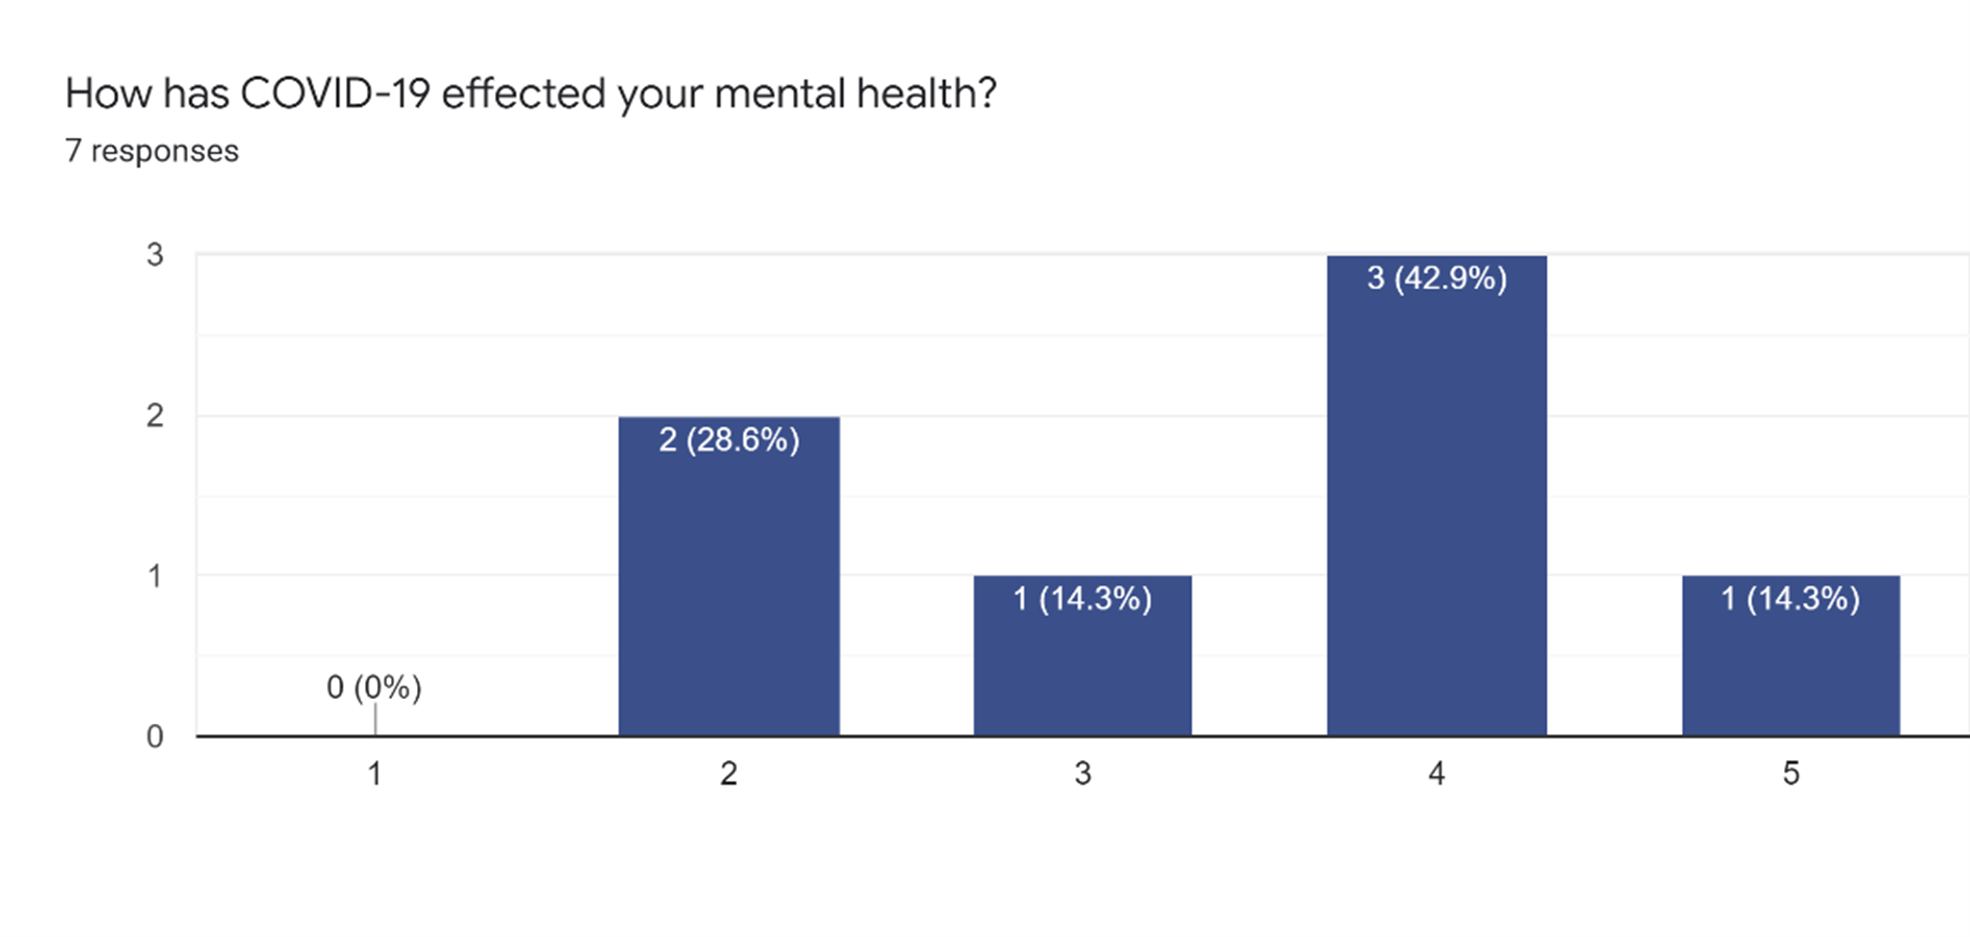
\includegraphics[width=100mm]{dissertation/images/gen.png}
     \caption{Participant's Mental Health}
     \setlength{\belowcaptionskip}{-10pt}
     \label{fig: Forms of exercise}
 \end{figure}
 
The full anonymized results can be found in \ref{Appendix C}. The physical activity of the participants before the COVID-19 The physical activity level of participants were gathered: sedentary is defined as less than 30 minutes of regular daily activity, somewhat active is defined as 30-60 minutes of regular daily activity, and active is defined as over 60 minutes of regular daily activity. Before the COVID-19 pandemic, 57\% of participants were classified as sedentary, and 42\% were classified as somewhat active. After the COVID-19 pandemic, the physical activity of participants decreased, with 85\% being classified as sedentary and 14\% being classified as somewhat active. Participants were asked what effect COVID-19 had on their mental health: 0\% noted a highly positive effect, 28\% noted a positive effect, 14\% noted a neutral effect, 42\% noted a negative effect, and 14\% noted a highly negative effect. 

\subsection{Study Results} 


\begin{figure}
\centering
\begin{subfigure}{.50\textwidth}
  \centering
  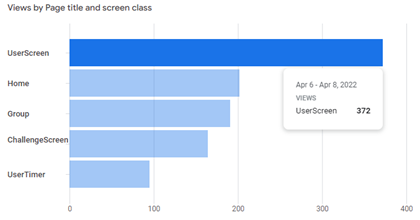
\includegraphics[width=\linewidth]{dissertation/images/20.png}
  \caption{Views Per Screen}
  \label{fig:sub1}
\end{subfigure}%
\begin{subfigure}{.5\textwidth}
  \centering
  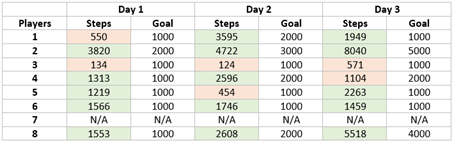
\includegraphics[width=\linewidth]{dissertation/images/21.png}
  \caption{Player's Step Count Data}
  \label{fig:sub2}
\end{subfigure}
\caption{A Initial questionnaire to gather requirements}
\label{fig:test}
\end{figure}
 
 
\textbf{Figures 6.5} summarise the data collected through the 3-day evaluation of the mobile application. This data was collected using the Google Analytics and Forage analytics tool. The user activity screen was the most visited, followed by the map and team screens. Note that the user timer screen is the fifth most visited screen; however, this does not consider that the timer can run in the background. Both teams succeeded in surviving the three days of the evaluation during the evaluation. In \textbf{Figure 6.5 (b)}, the step data highlighted green means the player had reached their step goal, while the orange step data meant that users did not meet their fitness goal. During the post-interview, player three and player four both reported that, on occasion, they accidentally closed the application during a workout meaning their steps were not recorded. 

\subsection{Warwick-Edinburgh Mental Wellbeing Scale Results} 
   \begin{figure}[h]
    \centering
     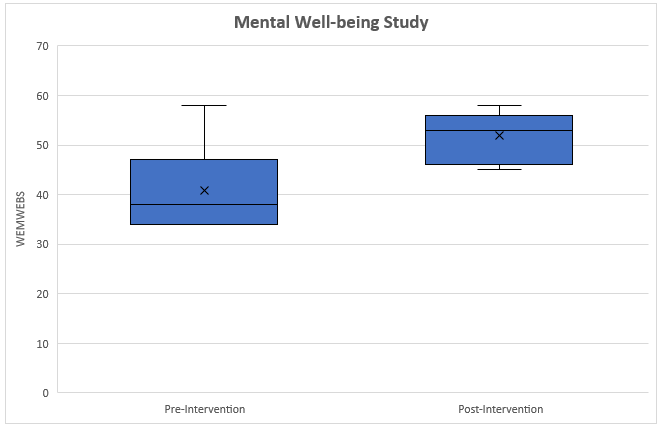
\includegraphics[width=120mm]{dissertation/images/22.png}
     \caption{Summary of WWEMWEBS Results}
     \setlength{\belowcaptionskip}{-10pt}
     \label{fig: Forms of exercise}
 \end{figure}
A summary of the results can be found in \textbf{Figure 6.6}, and the full results of the survey can be found in \ref{Appendix B}. Participants scored on average 40 points before the intervention and scored on average 51 points after the intervention. For the alternative hypothesis, it was predicted that participants would demonstrate an increase in their mental wellbeing score after using the Thrive mobile application. This hypothesis was formed from conducting the background research in chapter 2. The null hypothesis predicts that no significant change will occur to the mental wellbeing scores of participants after using the mobile application. To test the null hypothesis, a one-tailed paired sample t-test was applied for the statistical analysis of the one-sample group results. Using a one-tailed t-test means that the results would be more statistically significant compared to a two-tailed t-test. The t-value was calculated to be 4.5212, with a P-value of 0.001627. The p-value is lower than 0.05 and rejects the null hypothesis that states there is no meaningful change difference in the WEMWEBs scores after using the mobile application. 


\subsection{System Usability Scale Results} 
After the three-day evaluation, data were collected to evaluate the overall perceived usability of the mobile application. This was assessed using the popular Likert style questionnaire developed by John Brooke [\citenum{31}]. The SUS questionnaire contains ten questions that score a system between 0 and 100 by scoring elements such as the complexity and ease of use. Systems that score above 68\% are considered to have good usability, while a score below 68\% signifies the usability is below average. For Thrive, participants rated the application's usability very highly, with the system achieving a mean score of 89\%.
  
  
\subsection{Post-study Interview} 
To analyze the results from the interview, the transcript was broken down into codes and then grouped into themes. Overall, participants had a positive experience using the mobile application. 

\textbf{Health benefits}\vskip 0.5em
During earlier research conducted for the Background chapter, one paper discussed how the government’s quarantine measures led to an inadvertent increase in unhealthy behaviors. This was interesting as, during the interview, two players noted that having to walk outside led to inadvertent positive behaviors. Player 3 said that taking breaks from her work desk and doing something positive led her to take more time out for herself and her hobbies. Player 1 said, “It forced me to think about other people and be outside the little bubble you are in cause of COVID.” 

\textbf{Competitive }\vskip 0.5em
Different players showed different levels of competitiveness. Some players commented that they focused less on the team activity page that acted as a leader board and more on their individual step goals. Player 6: "I am not very competitive, so I did not pay much attention." Player 8 noted how even though he did not have the highest step count, he focused his competitiveness on the mini-challenges instead. This is the same with Player 1, stating that the mini-challenge's short interval made her push herself further. Other players enjoyed the leader board and mini-challenges due to their competitiveness. Player 2 said: "My team did not walk as much, so I had to do more, which had a positive effect because I did more." He commented that he would check the team's activity, and if he saw they would not survive the night, he made an extra effort to ensure they would. He found it appealing that he was able to check the step data of other users to ensure he would place it first on the activity screen, and he said. 

\textbf{Social  }\vskip 0.5em

Players commented that playing with people they knew in real life would have made the game more competitive. This was also found to be the case for the previous social fitness trackers researched in chapter 2. Additionally, Player 6 said she would have been more invested in the outcome of the mini-challenges had she been playing with friends. 

\textbf{Feedback  }\vskip 0.5em
Most participants noted that the XP feature could be extended so that the points gathered could be utilized to gain rewards. This would incentivize players to continue using the application by rewarding long-term participation. 
I had expected more comments about the sensitivity of the step counter; however, while some players noted it was somewhat sensitive, they stated that this is better than a step counter that does not count correctly. 
Players noted that they did not correctly record their steps due to forgetting to press the stop button after a walking session. A player noted that her habit of closing applications running on her phone led to her accidentally swiping the application away. Some players noted that the application could be improved by automatically recording their steps for convenience. 
Players that uploaded images to Firestore found that their profile picture would turn to one color and not display correctly after some time. 


\section{Discussion } 
\textbf{Initial survey and the general survey    }\vskip 0.5em
The results from the survey conducted during the evaluation asking about the impact of the COVID-19 pandemic are similar to the findings of the initial survey collected from a larger sample. Both surveys found that the pandemic had a 40\% increase in people experiencing a negative impact on their mental wellbeing. Moreover, both surveys showed there had been an increase in sedentary behavior. 
The results show that before COVID-19, there was an underlying issue of a high percentage of adults not doing enough regular physical activity in a week, leading to them being classified as sedentary. This behavior has only gotten worse, and there has been a considerable rise in people being classed as sedentary after the COVID-19 pandemic. 
It means effective measures need to be taken and be continued by both individuals and administrations to respond to sedentary behavior in public, especially in the aftermath of the pandemic. Doing so would improve an individual's overall mental and physical wellbeing. Accomplishing this would significantly benefit the healthcare system under stress from COVID-19 patients and the ongoing mental health crisis. The results from the general survey asking about the impact of the COVID-19 pandemic are similar to the findings of the initial survey collected from a larger sample. Both surveys found that the pandemic had a 40\% increase in people experiencing a negative impact on their mental wellbeing. Moreover, both surveys showed there had been an increase in sedentary behavior. 
The results show that before COVID-19, there was an underlying issue of a high percentage of adults being classified as sedentary by not doing enough regular physical activity in a week. This behavior has only gotten worse, and there has been a considerable rise in people being classed as sedentary after the COVID-19 pandemic. 
It means effective measures need to be taken and be continued by both individuals and the administration to respond to sedentary behavior in public, especially in the aftermath of the pandemic. Doing so would improve an individual's overall mental health and physical wellbeing, which has greater implications for the healthcare system under stress from COVID-19 patients and the mental health crisis. 


\textbf{User Study  }\vskip 0.5em
The user evaluation set out to prove the hypothesis that participants would see an increase in their mental well-being by using the fitness tracker to encourage physical activity. This was indeed found to be the case; a statistically significant increase was seen in participants' mental wellbeing scores. These results support earlier research that supporting regular physical activity in an individual lead to a positive impact on their mental wellbeing. Moreover, it was seen that by supporting physical activity, individuals started to adopt other self-care habits. The overall application was scored to be highly usable after a short period of time, meaning that following usability guidance was practical. 

\section{Future Work  } 
The evaluation can be improved by conducting a longer user study with a larger sample of participants to study the long-term effects of using Thrive. This would improve the validity of the results and mean that they could be generalized beyond the study. While the user evaluation found a statistically significant increase in mental wellbeing, this does not mean that the results are clinically significant. Further work can be conducted to see if the increase in mental wellbeing is clinically significant. This will show if the mobile application is a valid way to improve mental wellbeing instead of other techniques.   
The mobile application could be configured for iOS devices so that the user group is not limited to those with an Android device. In the user study, a participant could not take part due to their device being a newer model. Their phone’s security meant that it would only allow mobile applications published in the app store to be used. The system architecture could be improved by including Cloud Storage. This would mean that images uploaded by players could be saved to dedicated storage to fix the issue of images getting corrupted. 


\chapter{Conclusion}
\section{Summary} 
The mobile application Thrive achieved the goals it set out to accomplish at the beginning of the project. It offers a way to support an individual exercise in a collaborative setting to achieve individual and cooperative goals. The game implemented goal setting and offering rewards to support behavioral changes. It has been shown that the application is usable and engages users with its theme. That being said, the mobile application could be improved further to support behavioral changes such as implementing long-term rewards.
The collaborative environment supported the physical activity by players feeling compelled to exercise more due to their competitiveness or not wanting to let their team down. In this environment, players felt connected to people in their team. This contrasts with the environment COVID-19 had created- an environment where people felt disconnected and isolated in their bubble. 
It has been proven that this mobile fitness application, used to promote regular physical activity, is an effective way to improve the mental wellbeing of an individual. This supports the positive relationship between mental and physical wellbeing. This is an important finding, as maintaining these has positive long-term benefits, such as decreasing chronic disease, and short-term benefits such as potentially reducing the impact of COVID-19 and improving sleep habits. 

%==================================================================================================================================
%
% 
%==================================================================================================================================
%  APPENDICES  

\begin{appendices}


\chapter{Appendices}

\section{Initial questionnaire} \label{Appendix A}
\href{https://forms.gle/qxv14NxUnu199pyf6} {Link to Initial questionnaire} \vskip 0.5em
\href{https://docs.google.com/spreadsheets/d/10B9QG61xS7fSeA2y2isQTuKC0ugk30TObXXzkWz_L1Q/edit?usp=sharing}{Initial questionnaire anonymized data} \vskip 0.5em
 

\section{Prototype} \label{Appendix B}
\href{https://www.figma.com/file/h4xdbxNC4vys0PDbZfsxjT/FINAL-FIGMA-PROTOTYPE}{Link to Final Figma Prototype Desing}\vskip 0.5em
\href{https://forms.gle/wjo9DvXrN42DbPN28}{Link to Prototype consent form}\vskip 0.5em
\href{https://forms.gle/Cm9qfu1hV7dpEjji9}{Link to Prototype survey}\vskip 0.5em

\section{User Evaluation} \label{Appendix C}
 \href{https://gla-my.sharepoint.com/:b:/g/personal/2334016l_student_gla_ac_uk/EfHUC7LpK1dHsKLHslFcwI0BmL_7e_XV8HxEkXfQZNpKSw?e=iVjHoJ}{Link to Participation information sheet}\vskip 0.5em
 
\href{https://forms.gle/DYCryhi1vpAmYP1k9}{User study consent form}\vskip 0.5em
\href{https://docs.google.com/forms/d/1vpEoZpQgZi_qibabj_4qtD19afcUIP1_ZXTZ3_Ac3IE/edit}{User study general form}\vskip 0.5em
\href{https://docs.google.com/spreadsheets/d/1p5a72c8huqwutRpnsDH1Pz2NOcHlHbip-laDwR2N5BQ/edit?usp=sharing}{Link to General Questionnaire (anonymized Responses)}\vskip 0.5em

\href{https://forms.gle/oj8x8tqAieztgudd8}{Link to Pre-user study mental wellbeing form}\vskip 0.5em
 
\href{https://forms.gle/E6caHF4dPMYq1Pg69}{Link to Post-user study mental wellbeing form}\vskip 0.5em

\href{https://gla-my.sharepoint.com/:x:/g/personal/2334016l_student_gla_ac_uk/EZVaI_GVD6ZDq3rB-EB-uLYBnl6Swfg5YA_8EPg2bjBBnQ?e=fXcKd7}{Link to WEMWEBS Anonymized Data}\vskip 0.5em
\href{https://forms.gle/pfKHKZ2bkKx6tqtL9}{Link to SUS survey}\vskip 0.5em
\href{https://gla-my.sharepoint.com/:x:/g/personal/2334016l_student_gla_ac_uk/EXcE2XWkGkZNuWaiNeRZsNIBf1Bq9U0EtIrSveb6F3sIQQ?e=2ejXst}{Link to Interview Transcripts}\vskip 0.5em


 
 \section{Ethics Form} \label{Appendix D}
 \href{https://gla-my.sharepoint.com/:b:/g/personal/2334016l_student_gla_ac_uk/Ebww_bsl76hIrk1scK7UMY4BqAbai06eKcH8sILtsdYciQ?e=wl1Vo6}{Link to Ethics Form:}\vskip 0.5em

 \section{GitHub Repository} \label{Appendix E}
  \href{}{GitHub Repository Link}\vskip 0.5em
 






\end{appendices}

%==================================================================================================================================
%   BIBLIOGRAPHY   

% The bibliography style is abbrvnat
% The bibliography always appears last, after the appendices.

\bibliographystyle{plain}
\bibliography{l4proj.bib}



\end{document}
